\documentclass[a4paper]{book}

\usepackage[ngerman]{babel}								%Sprache
\usepackage[ansinew]{inputenc}						%Umlaute ohne Maske
%\usepackage{amsmath}											%Mathe f�r alle!
%\usepackage{amsfonts}											%Mathefonts
\usepackage{graphicx}											%Bessere Grafikunterst�zung
\usepackage[pdfborder = 0 0 0]{hyperref}	%Nette PDFs ohne M�h...


\title{PPLT-Handbuch}
\author{Hannes Matuschek\\ \texttt{hmatuschek@gmx.net}}
\date{2005-06-13}


\begin{document}
%	\begin{titlepage}
%		\maketitle
%		\vfill
%		\tableofcontents
%	\end{titlepage}
	\parindent = 0em
	\parskip = 2ex
	%\pagestyle{}
	
%\chapter{Einf�hrung}
%	\section{Was ist PPLT?}
	PPLT steht f�r \textit{Potsdamer Prozessleit-Technik} in Anlehnung an die 
	\textit{\index{Achener Prozessleittechnik}Achener Prozessleittechnik}
	\footnote{\href{http://www.acplt.de}{http://www.acplt.de}}. 
	Die PPLT ist ein so genanntes Framework, f�r die Kommunikation mit 
	Industriesteuerungen,	Sensoren, Aktoren oder mit 
	Haus-Auto\-matisierungs\-technik.

	Das System ist quelloffen und ist unter der \index{GNU-GPL} GNU-GPL bezeiungsweise der 
	\index{GNU-LGPL} GNU-LGPL lizensiert.
	Die GPL\footnote{General Public License} sichert jedem Benutzter, dass die Quellen
	des Programmes ihm ohne Einschrenkungen zug�nglich gemacht werden. Wenn jedoch
	das Programm oder Teile davon ver�ndert oder in anderen Projekten verwendet werden,
	m�ssen diese wiederum unter der GPL ver�ffentlicht werden. Um dennoch die M�glichkeit
	zu bieten, dass die PPLT in anderen Projekten verwendet werden darf, sind die 
	Bibliotheken, die den Gro�teil von PPLT ausmachen, unter der 
	LGPL\footnote{Lesser oder Library General Public License} lizensiert. Dies 
	bietet die M�glichkeit Teile der PPLT auch in eigenen Projekten zu verwenden und diese
	dann unter einer bliebigen Lizenz\footnote{durchaus auch properit�re Lizenzen} zu
	ver�ffentlichen. 

	Geschrieben wurde die PPLT in der Programmiersprache \index{Python} Python. Diese ist �hnlich
	wie Java eine Umgebung mit der platfomunabh�nige Programme entwickelt werden
	k�nnen. Somit ist auch die PPLT ein platformunabh�niges System. Sie k�nnen es
	so unter Linux oder auch unter Windows und anderen Betriebssystemen verwenden,
	ohne dazu den Quellcode �ndern zu m�ssen.


	\subsection{Ziele}
	Ziel war es ein System zu entwickeln, mit dem die Zust�nde nur einer
	bestimmten Steuerung beobachtet\footnote{sprich ausgelesen} werden 
	k�nnen. 
	
	Wie der Zufall es wollte, enstand aber ein System,
	welches sich dadurch auszeichnet, gerade \textbf{nicht} f�r ein
	bestimmtes Ger�t entworfen zu sein, sondern sich nicht einmal auf
	eine bestimmte Ger�teklasse beschr�nken l�sst. So gibt es bis jetzt
	Module\footnote{Module sind mit Treiber vergleichbar.}, die Mobiltelefone,
	Oszilloskope und verschiedene Industriesteuerungen lesen und beeinflussen
	k�nnen. 
	
	Konzeptionell l�sst sich PPLT als \index{zentrale Schnittstelle}zentrale 
	Schnittstelle zwischen Applikationen wie zum Beispiel Visualisierungen und 
	Ger�ten\footnote{Aktoren, Sensoren, Steuerungen} betrachten. 
	
	\begin{figure}[ht]
		\centering
		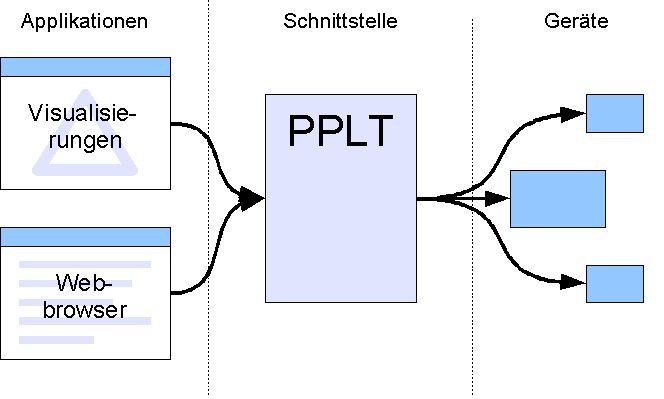
\includegraphics[scale=0.5]{ZieleGrenzen01}
		\caption{PPLT als Schnitstelle zwischen Applikationen und Ger�ten.}
		\label{fig:WiPPLT1}
	\end{figure}
	
	An einer solchen Position, ist es durchaus sinnvoll eine M�glchkeit zu haben
	zu bestimmen, wer auf welche Ger�te wie zugreifen darf. Daf�r wird ein so 
	genanntes Rechtemanagement ben�tigt. Solch eine \index{Rechteverwaltung}
	Rechteverwaltung bietet die PPLT. Sie besteht aus einer eigenen 
	\index{Benutzerdatenbank} Benutzerdatenbank, in der die \index{Benutzer} 
	Benutzer in hieraischen \index{Gruppen} Gruppen organisiert sind. 
	Zur \index{Authentifizierung} Authentifizierung des einzelnen	Benutzers 
	sind dann Benutzername und ein \index{Kennwort} Kennwort n�tig. Auf diese 
	Weise l�sst sich der Zugriff auf die Ger�te regeln, indem einzelnen 
	Benutztern	oder ganzen Gruppen der Zugriff auf Ger�te explizit gew�hrt 
	oder verboten wird.
	
	Dazu ein Beispiel:\\
	In einem Unternehmen sind die R�ume klimatisiert. Die Klimaanlage als
	automatisierter Prozess soll von den Mitarbeitern moduliert werden k�nnen.
	Um zu verhindern, dass ein Mitarbeiter aus Versehen oder Absicht die 
	Klimanalage eines Fremden B�ros manipuliert, sollte jeder Mitarbeiter nur
	Zugriff auf die Klimaanlage seines eigenen B�ros haben. 
	
	Um mit m�g\-lichst viele verschiedenen Programmen zusammen arbeiten zu k�n\-nen,
	besitzt die PPLT die M�glichkeit, die Schnittstelle zu den Applikationen 
	auszutauschen. Diese Schnittstelle wird hier \textit{Server} genannt. 
	\index{Server}Server sind im Allgemeinen Programme, die ihre Dienste anderen 
	Programmen zur Verf�gung stellen. So kann also die Unterst�tzung f�r ein 
	bestimmtes Programm, w�rend der Laufzeit in die PPLT geladen	werden.
	
	Dazu ein Beispiel:
	M�chte man von unterwegs mit dem PDA/Handy oder im Internet-Cafe �berpr�fen,
	ob man vieleicht zu Hause bestimmte Ger�te versehentlich nicht ausgeschaltet
	hat, so empfiehlt sich die Steuerung der Haushaltsger�te mittels Webserver,
	da sich ein Webbrowser mittlerweile auf jedem Handy finden l�sst. Also
	wird ein Webserver in die PPLT geladen, �ber den man sp�ter, nach einer
	Authentifikation\footnote{Login}, die Haushaltsger�te, zur Not von �berall aus,
	abschalten kann.

	\subsection{Grenzen}
	Die PPLT unterliegt wie jedes Programm bestimmten Grenzen. Anhand dieser kann
	man erkennen wo sich die Software einsetzten l�sst oder viel mehr, wo diese 
	nicht	verwendbar ist.
	
	Die PPLT l�sst sich grunds�tzlich nur als Master innerhalb eines Buses ein
	setzten. Diese Restriktion gild aber nur f�r die Kommunikation mit den 
	Gr�ten. Die PPLT kann also keine Anfrage eines Ger�tes verabeiten und
	Beantworten. Anfragen, die an einen Server der PPLT gestellt werden,
	kann das System aber sehr wohl bearbeiten. 
	
	Diese unscheinbar wirkende Einschr�nkung hat jedoch gro�e Auswirkungen
	auf das Einsatztgebiet der PPLT. So l�sst sich das System nur bedingt
	in der industriellen Produktion verwenden. Das Hauptproblem bei der 
	�berwachung solcher Prozesse liegt in der Reaktionszeit. Die PPLT
	m�sste zur �berwachung eines Prozesses dessen Werte zyklisch abfragen.
	Dabei kommt es aber zu unn�tig hohem Datenverkehr, da die PPLT die 
	mei�te Zeit sich nicht �nderne Werte sammelt und so ggf. auf ein
	Erreignis zu sp�t reagieren k�nnte. Die PPLT ist also f�r das 
	Monitoring von Prozessen nur eigeschr�nkt nutzbar.
	
	Die St�rke der PPLT liegt, bedingt durch ihre Konstruktion, in der
	aktiven Rolle\footnote{Also nicht in der passiven �berwachung.}.
	Also zum Beispiel in der Modulierung\footnote{Manipulation} 
	automatisierter Prozesse.
	

%	\section{Funktionsweise}
	\begin{figure}[ht]
		\centering
		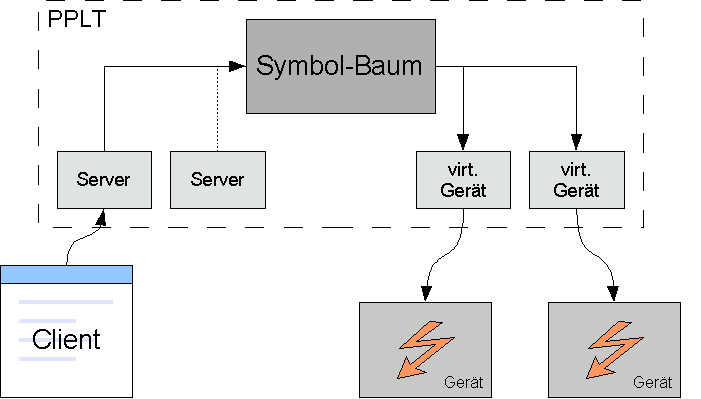
\includegraphics[scale=0.5]{ZieleGrenzen02}
		\caption{schematische Funktionsweise der PPLT}
		\label{fig:WiPPLT2}
	\end{figure}
	Wie in der Abbildung \ref{fig:WiPPLT1} ist auch in der 
	Abbildung \ref{fig:WiPPLT2} die PPLT als Schnittstelle zwischen den 
	Applikationen (Client) und den Gr�ten dargestellt. Hier jedoch,
	ist der interne Aufbau der PPLT augedeutet.
	
	Es ist ein regul�rer Ablauf einer Anfrage eines Clienten dargestellt:\\ Zun�chst
	stellt der Client eine Anfrage an den Server. Dieser verarbeitet diese und holt
	sich aus dem \textit{Symbolbaum} die zur Beantwortung ben�tigten Werte. Der 
	Symbolbaum, eine Art Mischung aus virt. Dateisystem und Wertetabelle, wiederum
	holt sich die Daten aus den virtuellen Ger�ten\footnote{Virtuelle Ger�te sind die 
	Repesentation der realen Ger�te innerhalb der PPLT. Man kann sich diese als
	\textit{Treiber} vorstellen.}. Die virtuellen Ger�te sind in der Lage mit den 
	realen Ger�ten zu kommunizieren. Sie tauschen also mit den realen Ger�ten Pakete aus
	und erhalten so die ben�tigten Informationen, die sie an den Symbolbaum zur�ckgeben.
	Dieser wandelt die erhaltenen Daten ggf. um und �bergibt diese als Wert dem Server.
	Der Server kann nun die gestellte Anfrage des Clienten beantworten.
	
	Ich m�chte nun ein wenig genauer auf die einzelnen Elemente der PPLT eingehen. Die 
	Abbildung \ref{fig:WiPPLT2} zeigt schon die 3 Hauptbestandteile der PPLT. Die Server,
	die Ger�te sowie der zentrale Symbolbaum.
	
	\subsection{Die virtuellen Ger�te}
	Die virtuellen Ger�te\footnote{Werden im folgenden nur noch \textit{Ger�te} genannt},
	sind wie schon erw�hnt in der Lage mit real existierender Hardware zu kommunizieren.
	Diese Ger�te sind jedoch nicht fester Bestandteil der PPLT. Sie werden je nach bedarf
	w�rend der Laufzeit geladen. Genauer gesagt, ist nach der Installation der reinen
	PPLT das System nicht in der lage mit irrgendeinem Ger�t zu kommunizieren. Dies wird
	erst durch das Installieren der Module\footnote{Ger�tedateien} m�glich. Jedes dieser 
	Module erweitert die F�higkeiten des Systems. 
	
	Ich m�chte an dieser Stelle nicht verschweigen, dass ein Ger�t mei�t aus mehreren 
	so genannten Kernmodulen besteht. Dies ist sinnvoll, da zum Beispiel viele Ger�te die
	serielle Schnittstelle nutzen, k�nnen durch eine seperate Implementierung der seriellen
	Schnittstelle eine Vielzahl an Ger�ten dieses Kernmodul und damit die Schnittstelle 
	nutzen. Dies ist aber f�r das Verstehen der Funktionsweise nicht weiter wichtig.

	Die Ger�te geben, einmal geladen, dem System die M�glichkeit indirekt aus der
	realen Hardware zu lesen und/oder zu schreiben. 
	
	Ein einzelnes Ger�t kann jedoch viele verschiedene Werte liefern. Ein gutes Beispiel
	hierf�r ist eine Industriesteuerung. Sie mehrere Ein- und Ausg�nge, eine Vielzahl an
	Registern, Z�hlern und Zeitgebern. F�r jeden dieser einzelnen Werte besitzt ein Ger�t
	einen so genannten Slot\footnote{Buchse, Anschluss}. Verbindet man etwas mit diesem
	Slot, so kann man auf den etsprechenden Wert zugreifen.
	
	\subsection{Der Symbolbaum}
	Der Symbolbaum ist wie ein Dateisystem aufgebaut. Er kennt Verzeichnisse\footnote{Ordner},
	in denen zwar keine Dateien aber Symbole abgelegt werden k�nnen. Ich werden an dieser
	Stelle nicht weiter auf die Verzeichnisse eingehen sondern das Augenmerk auf das Symbol
	legen:

	\begin{itemize}
		\item Ein Symbol representiert einen Wert. So kann ein Symbol eine gemessene Temperatur
		oder den Fullstand eines Tanks in Prozent wiedergeben. 
		\item Ein Symbol representiert einen bestimmten Wert eines bestimmten Gr�tes. So kann
		ein Symbol die Eing�nge einer Steuerung representieren. Wenn aus diesem Symbol gelesen 
		wird, erh�lt man die dort anliegenden Signale.
		\item Ein Symbol ist mit einem Ger�t fest Verbunden, genauer gesagt ist es mit einem Slot 
		eines Ger�tes verbunden. Das Ger�t kann nicht entladen\footnote{gel�scht/entfernt} werden, 
		solange ein Symbol mit im	verbunden ist.
		\item Ein Symbol hat einen Bestimmten Typ. Dieser kann Bool, Byte, Word, 
		DWord\footnote{Doppelwort}, Float, Double oder String sein.
	\end{itemize}
	
	\begin{figure}[ht]
		\centering
		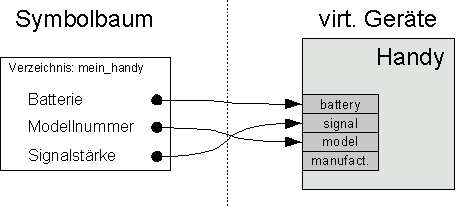
\includegraphics[scale=0.6]{Symbol01}
		\caption{Verbindung zwischen Symbolen und Ger�ten}
		\label{fig:funkt1}
	\end{figure}
	
	In der Abbildung \ref{fig:funkt1} ist die Verkn�pfung der Symbole aus dem Symbolbaum
	mit den Slots eines Ger�tes dargestellt. \texttt{Batterie}, \texttt{Modellnummer} und
	\texttt{Signalst�rke} sind Symbole im Verzeichnis \texttt{mein\_handy} des Symbolbaumes.
	\texttt{battery}, \texttt{signal}, \texttt{model} und \texttt{manufact.} sind 
	Anschl�sse des Ger�tes \texttt{Handy}.	
	
	Wenn sie nun aus dem Symbol \texttt{Batterie}
	lesen, erhalten sie den Wert, des Anschlusses \texttt{battery} des Ger�tes 
	\texttt{Handy}. Ebenso verh�lt es sich beim Schreiben. Wenn sie in ein Symbol schreiben,
	schreiben sie damit in den Anschluss des dazugr�rigen Ger�tes.
	
	Ich m�chte an dieser Stelle noch erw�hnen, dass die Symbole und die Verzeichnisse in
	der PPLT einem Benutzer und einer Gruppe zugeordnet sind. Des weiteren lassen sich
	Zugriffsrechte f�r die Symbole und Verzeichnisse vergeben. Auf diese Weise kann 
	der Zugriff auf die Ger�te oder besser auf dessen Werte reguliert werden. 
	
	\begin{figure}[ht]
		\centering
		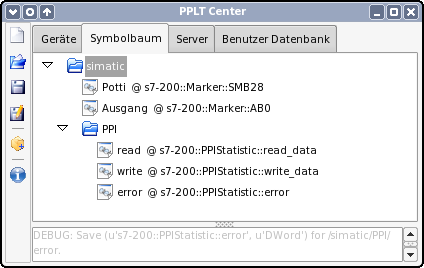
\includegraphics[scale=0.5]{PPLTC7}
		\caption{Der Symbolbaum in der PPLT-Center Applikation.}
		\label{fig:funct2}
	\end{figure}
	In der Abbildung \ref{fig:funct2} ist das Fenster der PPLT-Center Applikaion, welches
	den Symbolbaum darstellt, zu sehen.
	
	\subsection{Die Server}
	Server sind wie die Ger�te ladbare module. Ein Server kann also w�rend der Laufzeit 
	gestartet oder angehalten werden, ohne das Programm beenden zu m�ssen. Ihre Aufgabe 
	ist es die Werte im Symbolbaum zu exportieren und so anderen Applikationen zur
	Verarbeitung\footnote{Zum Beispiel zur Darstellung in einer Visualisierung} zur
	Verf�gung zu stellen. 
	
	Ein Beispiel hierf�r ist ein ladbarer Webserver, der
	den Symbolbaum f�r einen Webbrowser aufarbeitet. Auf diese Weise kann der 
	Symbolbaum mit einem Browser durchsucht und die darin enthaltenen Werte
	ausgelesen werden.
	
	Dabei ist zu bemerken, dass ein Server nicht unbedingt den Ganzen Symbolbaum
	exportieren muss. Man kann das System anweisen, das ein Bestimmter Server
	nur einen Teilbaum, zum Beispiel nur ein einzelnens Verzeichnis exportieren
	soll.
	
	\begin{figure}[ht]
		\centering
		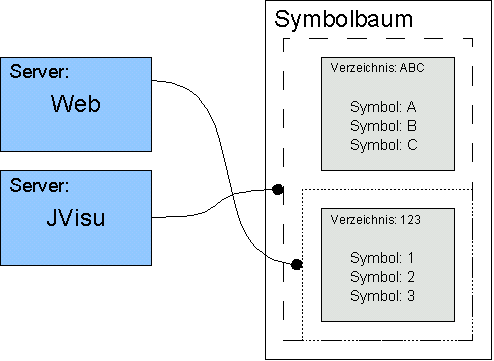
\includegraphics[scale=0.5]{Server01}
		\caption{Server exportieren den Symbolbaum oder Teile davon.}
		\label{fig:server1}
	\end{figure}
	
	In Abbildung \ref{fig:server1} ist folgende Situation dargestellt. Zwei Server
	exportieren Teile des Symbolbaums. Der erste Server, ein Web-Server, exportiert jedoch
	nur einen Teilbaum n�mlich das Verzeichnis \texttt{123}. Anders als der Web-Server
	exportiert der JVisu-Server\footnote{Ein Server, aus den die Visualisierung \texttt{JVisu}
	ihre Daten beziehen kann.} die Verzeichnisse \texttt{123} sowie \texttt{abc}, also
	den gesammten Symbolbaum. Es ist also nicht m�glich �ber den Webserver auf Symbole im
	Verzeichnis \texttt{abc} zugreifen. Auf diese Weise k�nnen vertrauensunw�rdige Dienste
	auf unkritische Abschnitte des Symbolbaums beschr�nkt werden.	

%\chapter{Installation}
%	\section{Was ben�tige ich?}
	Um die PPLT benutzen zu k�nnen, m�ssen eine Reihe Bedingungen erf�llt sein. Sie ben�tigen
	zu aller erst den Python-Interpreter, da die PPLT in dieser Scriptsprache geschrieben wurde.
	Diesen Interpreter ist quelloffene Software und kann kostenlos von der URL
	\href{http://www.python.org}{www.python.org} heruntergeladen werden. Sie ben�tigen 
	jedoch Python ab der Version \textbf{2.3.0}.
	
	Wenn sie die grafische Applikation PPLT-Center (\texttt{PPLTC}) verwenden wollen, ben�tigen sie
	die wxPython Bibliothek. Diese Bibliothek erm�glicht die platform�bergreifende Programmierung von
	grafischen Benutzterprogrammen. Diese ist ebenso wie Python eine Quelloffene Bibliothek, die sie
	von der URL \href{http://www.wxpython.org}{www.wxpython.org} herunterladen. Da sich die 
	API der Bibliothek ver\-�ndert hat, ben�tigen sie mindestens die recht aktuelle Version 
	\textbf{2.5.0}. Zu beachten ist, dass sie diese Bibliothek nicht ben�tigen, wenn sie die 
	Applikation \texttt{PPLTC} nicht verwenden m�chten.
	
	Wenn sie das Betriebssystem \textbf{Windows} von Microsoft verwenden, sollten sie auf jeden
	fall die Python-Bibliothek pywin32 herunterladen. Diese ist ebenso quelloffen und ist unter
	der URL \href{http://pywin32.sourceforge.net}{pywin32.sourceforge.net} herunterladen. 
	Dieses Projekt verfolgt eine recht eigensinnige Versionsnummerierung. Die ben�tigen 
	mindestens die Version \textbf{203}. Wenn sie jedoch	\textbf{Posix} 
	kompatible\footnote{Linux, Unix, HP-UX, BSD, ...} Betriebssysteme verwenden,
	ben�tigen sie diese Bibliothek nicht.
	
	Es kann durchaus vorkommen, dass ein bestimmtes Kern-Modul eine weitere, nicht in der Standard
	Bibliothek enthaltene, Bibliothek ben�tigt. Dies entnehmen sie bitte der der Dokumentation des
	einzelnen Moduls. Ich einieger Voraussicht laden sie bitte die Bibliothek
	pyserial von der URL \href{http://pyserial.sourceforge.net}{pyserial.sourceforge.net}
	herunter. Diese Bibliothek bietet eine Platform\-�bergreifende M�glichkeit die serielle 
	Schnitstelle zu nutzen. Diese Bibliothek wird von der Kern-Bibliothek \texttt{UniSerial} 
	verwendet, welches selber	wieder von einer Vielzahl von Ger�ten verwendet wird.
	
	An dieser Stelle m�chte ich anmerken, dass f�r die ersten Versuche mit der PPLT keinerlei
	besondere Hardware von N�ten ist. Dementsprechend sind die Beispiele aber etwas 
	unspektakul�r. Sie beschr�nken sich auf das erzeugen von Zufallswerten.

	\subsection{Installation der Software}
	Ich kann ihnen an dieser Stelle keine vollst�ndige Installationsanleitung
	f�r diese Pakete anbieten. Dies w�rde den Rahmen dieses Dokumentes Spr�ngen.
	
	Dennoch will ich ihnen hier eine kurze "`Schritt f�r Schritt"'-Anleitung 
	zur Installation geben. Die Installation der PPLT wird im n�chsten Abschnitt 
	besprochen.
	
	\subsubsection{Unter Windows}
		Die Installation von Python, wxPython und der pywin32 Erweiterung d�rfte sich 
		unter Windows recht	Problemlos gestalten. F�r all diese Pakete gibt es so
		gennte Installer. Dies sind ausf�hrbare Dateien\footnote{Unter Windows *.exe},
		die den Installationsprozess automatisieren. Nach dem Starten eines solchen
		Installers �ffnet sich ein Dialog, der die f�r die Installation ben�tigten
		Eingaben abfragt. Mei�t k�nnen sie die dort stehenden Standard Werte �bernehmen.
		
		Bei der Installation von Python wird am Anfang das Verzeichnis abgefragt, in
		das Python installiert werden soll. (Siehe Abbildung \ref{fig:PyInstall})
		Bitte merken oder notieren sie sich dieses Verzeichnis, es wird sp�ter 
		ben�tigt um die Dateien der PPLT wieder zu finden. 

		\begin{figure}[ht]
			\centering
			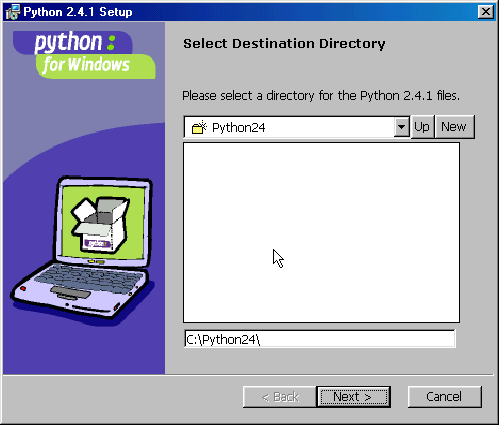
\includegraphics[scale=0.5]{PythonInstall}
			\caption{Python Installer}
			\label{fig:PyInstall}
		\end{figure}
		
		In diesem Verzeichnis	liegt auch die ausf�hrbare Datei des Python-Interpreters. 
		Bitte �ffnen sie jetzt eine Eingabeaufforderung und geben sie \texttt{python}
		ein. Nun sollte sich die Python-Konsolle �ffnen\footnote{Mit Strg-Z beenden die
		die Konsole}. Ist dies nicht der Fall und sie erhalten einen Fehler, dass
		dieser Befehl unbekannt sei, m�ssen sie Windows mitteilen, dass es auch in 
		dem oben erw�hnten Verzeichnis nach ausf�hrbaren Dateien suchen soll.
		
		Dies k�nnen sie unter Windows95/98 mit einem Text-Editor oder dem Programm
		\texttt{msconfig} erledigen. Editiren sie die 
		\texttt{autoexec.bat}\footnote{Mei�t dierekt auf dem Laufwerk \texttt{C:}}
		und f�gen sie die Zeile \texttt{set PATH=\%PATH\%;C:$\backslash$Python24$\backslash$} 
		hinzu\footnote{Bitte ersetzen sie C:$\backslash$Python24$\backslash$ mit dem Verzeichnis, in das
		sie Python installiert haben.}.
		
		Unter Windows 2000/XP gestaltet sich dieser Eintrag einfacher. �ffnen sie
		bitte \texttt{Systemsteuerung->System}\footnote{Bitte beachten sie, dass sie unter
		Windows 2000/XP als Systemadministrator angemeldet seien m�ssen}. W�hlen sie den Reiter 
		\texttt{Erweitert} aus und klicken sie auf \texttt{Umgebungsvariablen}.
		Es �ffnet sich ein Fenster indem sie die Umgebungsvariablen f�r den 
		aktuellen Benutzer und das System setzen k�nnen. Unter den Systemvariablen
		befindet sich auch die Variable \texttt{Path}. W�hlen sie diese aus und
		klicken sie auf \texttt{Bearbeiten}. F�gen sie bei \texttt{Wert der Variablen}
		\texttt{;C:$\backslash$Python24$\backslash$} hinzu, oder eben das Verzeichnis, in das sie Python
		installiert haben.
		
		Bitte beachten sie das Semikolon. Wird dieses vergessen, kann das das Verhalten
		anderer Programme beeinflussen.
		
		Bitte beachten sie, dass sie \textbf{zuerst} Python und \textbf{dann} 
		wxPython und pywin32 installieren.
		
		Die Installation von pyserial k�nnte sich etwas schwierieger gestalten, da
		f�r dieses Packet nicht unbedingt ein Installer vorliegt. Ist dies nicht der
		Fall, laden sie bitte das Quellarchiv herunter und entpacken es. 
		
		Starten sie dann eine Konsole\footnote{MS-DOS Eingabeaufforderung} und
		wechseln sie mit \texttt{cd} in das Verzeichnis, das sie entpackt haben.
		
		F�hren sie nun \texttt{python setup.py install} aus\footnote{Achten sie bitte auf
		die Leerzeichen}. Nun sollte die Bibliothek installiert werden. 
		
	\subsubsection{Unter Posix}
		Die Installation der Software unter Posix-Systemen wie Linux, Unix oder BSD gestaltet sich 
		von Anbieter zu Anbieter recht unterschiedlich. Am einfachsten ist es, wenn der Distributor
		die ben�tigte Software als Inastallationspakete\footnote{Zum Beispiel als RPM oder DEB Dateien} 
		im Bin�rformat anbietet. Python und wxPython werden bei den gro�en Distributionen mitgelifert.
		Aktuelle Distributionen d�rften auch die neueren Pakete, also in der aktuellen Version, enthalten.
		Jedoch ist in der SuSE 9.1 Distribution eine zu alte Version von wxPython enthalten, so dass diese
		aktualisiert werden sollte.
		
		Am sichersten sind sie, wenn sie die Quellen von Python sowie wxPython heunterladen und
		selber kompalieren. Dies sei aber nur erfahreren Benutzern empfohlen.
		
		F�r die Linux Distributionen Debian und Red Head liegen auch fertige Bin�r-Installationspackete
		auf dem Servern von Python und wxPython. Diese sollten sich mit dem Paketmanager der jeweiligen
		Distribution problemlos installieren lassen.
		
		Zur installation den pyserial Bibliothek empfiehlt es sich die Quellen\footnote{Mit der Endung 
		\texttt{tar.gz} oder \texttt{tar.bz2}} herunter zu laden. Dieses Archiv enth�lt ein 
		Installationsscript, mit dessen Hilfe die Installation sehr einfach durchgef�hrt werden kann.
		
		Wechseln sie auf eine Konsole und gehen sie in das Verzeichnis, indas sie das Archiv gespeichert haben.
		Entpacken sie das Archiv mit: 
		
		\texttt{tar -x?? pyserial-???.tar.gz} 
		
		Es sollte nun ein neues
		Verzeichnis mit dem Namen \texttt{pyserial-???} im aktuellen erzeugtworden sein. Wechseln sie
		in dieses Verzeichnis und f�hren sie:
		
		\texttt{python setup.py install} aus.
		 
		Nun wird die Bibliothek installiert.
		
		Sind alle erw�hnten Softwarepakete installiert, k�nnen sie mit der Installation der PPLT
		beginnen. Sollten bei der Installation Probleme auf treten oder wenn sie Fragen zu diesem
		Text haben, wenden sie sich bitte per E-Mail an mich.
		
%	\section{PPLT Installieren}
	\subsection{PPLT Center}


%\chapter{Konfiguration}
%		Obwohl es f�r eine Bibliothek ungew�hnlich ist, eine Konfiguration zu besitzen, lassen sich
	bei der PPLT in guter Posix-Manier, einige Einstellungen mittels einer Konfigurationsdatei t�tigen.
	
	Die Eistellm�glichkeiten sind aber eher bescheiden, so dass dieses Kapitel eher kurz werden
	d�rfte. Eigentlich lassen sich nur ein paar Verszeichnisse, in denen das System
	nach Modulen und Icons suchen soll, die Sprache und die so genannten LogLevel
	einstellen.
	
	Wie schon oben erw�hnt, besitzt die PPLT eine Konfigurationsdatei. Diese kann mit einem
	Texteditor manipuliert werden. Dem routinierten Windowsbenutzer d�rfte diese Art der 
	Konfiguration ungewohnt erscheinen. Wo hingegen Anwender mit Linux-Erfahrung dar�ber
	m�de l�cheln. 
	
	Die Konfigurationsdatei befindet sich in dem Verzeichnis, in dem die PPLT all ihre Daten,
	wie die Icons f�r das PPLT-Center oder eben die Module ablegt. Dieser Ordner hei�t 
	\texttt{PPLT} und liegt unter Windows in dem Verzeichnis, in das sie Python installiert 
	haben. Unter Linux sollten sie einmal im Verzeichnis \texttt{/usr} oder \texttt{/usr/local}
	nachsehen. Die Datei hei�t \texttt{PPLT.conf}. �ffnen sie diese mit dem Texteditor ihrer wahl.
	
	Der Aufbau der Konfiguration ist recht einfach. In eckigen Klammern stehen die einzelnen
	Bereiche der Konfiguration. In der PPLT.conf w�ren das der Bereich \texttt{lang}
	in dem alle Einstellungen der Sprache betreffend gemacht werden k�nnen. Im Abschnitt
	\texttt{logging} k�nnen sie das Meldungsverhalten der PPLT beeinflussen. Im letzten
	Abschnitt \texttt{path} werden die Pfade f�r PPLT, wie zum Beispiel der Pfad zu den 
	Icons gesetzt.
	
	\section{Die Spache}
	In diesem Bereich k�nnen sie die Sprache der PPLT und vor allem die Spache des PPLT-Centers
	festlegen. Auff�llig ist, dass hier zwei Spacheintr�ge vohanden sind. Der erste Eintrag
	beschreibt die prim�re Sprache. Wenn sie also eine deutsche �bersetzung w�nschen,
	sollten sie bei \texttt{language:} \texttt{de} eintragen. 
	
	Der Eintrag \texttt{alt-lang} bedeutet soviel wie "`Alternativ Sprache"' dieser Eintrag
	wird dazu benutzt eine Sprache zu definieren, auf die zur�ckgereiffen werden soll, wenn
	die prim�re Sprache nicht verf�gbar ist. Deshalb sollten sie hier den Eintrag auf
	\texttt{en} belassen.
	
	Eine sinnvolle Sprachkonfiguration f�r die Sprache Deutsch w�re:
	\begin{verbatim}
[lang]
language: de
alt-lang: en
	\end{verbatim}
	
	
	\section{Das Logging}
	Als logging bezeichnet man Verarbeitung und Ausgabe von Nachrichten, die w�rend
	des Prgrammablaufes auftreten. Solchen Nachrichten haben verschiedene Gewichtungen
	und k�nnen von einfachen informativen Meldungen bis hin zu Fehlermedungen 
	klassifiziert werden. In diesem Abschnitt k�nnen sie festlegen welche Gewichtung 
	einen Meldung haben muss um �berhaupt verarbeitet zu werden. Meldungen 
	geringerer Gewichtung werden ignoriert. Des weiteren k�nnen sie festlegen, wie
	diese gefilterten Meldungen ausgegeben werden sollen. 
	
	\subsection{LogLevel}
	Die PPLT klassifiziert die Meldungen in \texttt{debug}, \texttt{info},
	\texttt{warning}, \texttt{error} und \texttt{fatal}. Wobei \texttt{debug}
	die niedrigste und \texttt{fatal} die h�chste Stufe darstellt. 
	
	Als \texttt{debug} werden all die Meldungen deklariert, die zur Fehlerfindung im
	Program hilfreich seien k�nnten. Dies sind aber sehr viele. So dass, wenn sie dieses
	Level ausw�hlen, sie sehr viele Meldungen erhalten. Daher ist diese Gewichtung
	f�r den normalen Betrieb eher ungeeignet.
	
	Als \texttt{info} werden informative Medungen deklariert, die durchaus f�r den Anwender 
	interresant sind. Es ist also sinnvoll diesen Filter f�r die Konfiguration zu verwenden.
	Setzten sie daher bitte in der Konfiguration:
	\begin{verbatim}
[logging]
CoreLevel: info
PPLTLevel: info
File: No
SysLog: No
	\end{verbatim}
	Damit werden Nachrichten mit der Gewichtung \texttt{info} oder h�her verarbeitet.
	
	Meldungen, mit der Gewichtung \texttt{warning}, stellen Warnungen dar. Diese Meldungen
	weisen gegenbenenfalls auf Fehlfunktionen hin. Jedoch deuten diese nich zwingend auf
	eine Fehlfunktion hin.
	
	Mit \texttt{error} oder \texttt{fatal} werden Nachrichten gewichtet, die auf einen
	Fehler hinwiesen. Jedoch bedeutet \texttt{fatal}, dass dieser Fehler aus einem Fehler
	im Programm und nich auf einer Fehlbedienung herr�ht. Tritt also ein Fehler mit der
	Gewichtung \texttt{fatal} auf, wenden sie sich bitte an den Autor.
	
	In der Konfiguartionsdatei finden sie zwei Level- oder Filter-Ein\-tr�ge. Der 
	Eintrag \texttt{CoreLevel} setzt den Filter f�r die Kernbibliothek. Der Filter
	f�r die PPLT-Bibliothek und das PPLT-Center kann mit dem Eintrag 
	\texttt{PPLTLevel} gesetzt werden. Es ist durchaus sinnvoll f�r beide Eintr�ge 
	die selben Filter zu verwenden.
	
	\subsection{Ausgabeumleitung}
	Es ist m�glich die Ausgabe der gefilterten Meldungen umzuleiten. Zum Beispiel in eine
	Datei oder zu einem Logging-System des Betriebsystems\footnote{Steht bis jetzt nur f�r 
	Posix-Systeme zur Verf�gung}. Dazu existieren die Eitr�ge \texttt{File} sowie
	\texttt{Syslog} in der Konfiguration. Wenn sie beide Eintr�ge auf \texttt{No} belassen,
	werden die Nachrichten auf der \texttt{StdErr} ausgegeben. 
	
	Wenn sie jedoch bei \texttt{File} den Pfad einer Datei angeben, werden die Meldungen
	in eben dieser Datei abgelegt. 
	
	Wenn sie \texttt{SysLog} auf \texttt{Yes} setzten, werden die gefilterten Nachrichten
	an den SysLog-D�mon des Betriebssystems\footnote{Existiert nur unter Posix Systemen.}
	gesendet. Diese Einstellung �berschreibt den \texttt{File}-Eintrag. Das bedeutet,
	wenn sie \texttt{SysLog} auf \texttt{Yes} gesetzt haben und eine Datei bei \texttt{File}
	angegeben haben, werden jedoch alle Meldungen ausschlie�lich an den SysLog-D�mon 
	gesendet.
	
	Eine sinnvolle Konfiguration w�re:
	\begin{verbatim}
[logging]
CoreLevel: info
PPLTLevel: info

File: No
SysLog: No
	\end{verbatim}
	
		
	\section{Pfadeinstellungen}
	\textbf{Achtung:} �nderungen an den Pfadeinstellungen sollten nur von erfahrenen Benutztern
	gemacht werden. Fehleinstellungen k�nnen das Verhalten des Programms starkt beeinflussen.
	
	Im Abschnitt \texttt{path} werden sie Pfade zu den Dateien, die die PPLT ben�tigt gesetzt.
	Dazu ge\-h�ren die Module, Ge\-r�te, Server, Icons und die Benutzer\-daten\-bank-Datei. 
	
	F�r alle Eintr�ge ist \texttt{AUTOMATIC} eine g�ltige Option. Damit sagen sie dem System,
	dass es die Standard-Pfade benutzen soll. 
	
	Mit \texttt{BasePath} wird der Pfad zu dem PPLT Verzeichnis, in dem sich auch die 
	Konfigurationsdatei befindet, gesetzt. Dem Eintrag \texttt{UserDB} �bergeben sie 
	die Benutzterdatenbank-Datei, somit ist es m�glich verschiedene Datenbanken f�r
	die PPLT zu unterhalten. Der Eintrag \texttt{DBPath} ist obsolet und setzt den Pfad auf
	das Verzeichnis, indem sich die Server- und Ger�te-Dateien befinden. Mit 
	\texttt{IconPath} wird der Pfad auf das Verzeichnis gesetzt, welches die Icons
	f�r das PPLT-Center beinhaltet.
	
	Bitte �ndern sie die Eintr�ge nur, wenn sie wissen was sie tun.

%\chapter{PPLT Center}
%	Im Kapietel "`Installation"' sind sie schon mit dem PPLT Center in ber�hrung gekommen. In diesem Kapitel
werde ich ihnen einen tieferen Einbick in die Funktionsweise und die Bedienung des PPLT Centers
geben. 

Doch zun�chst starten sie bitte die PPLT Center Applikation. Klicken sie auf den Reiter
"`Benutzer Datenbank"'. Die sehen dort das Symbol einer Gruppe diese hei�t \texttt{Admin}.
Mit einem Doppelklick auf dieses Symbol �ffnen sie diese Gruppe. In dieser Gruppe befindet 
sich lediglich ein Benutzer mit dem Namen \texttt{admin}. Das Symbol des Benutzers ist rot 
hinterlegt. Das bedeutet, dass dieser Benutzer der Superuser oder Administrator ist.
Sie sollten jetzt das Passwort des Administrators �ndern. Dazu �ffnen sie mit der
rechten Maustaste ein Kontextmenu und klicken auf "`Passwort �ndern"'\footnote{Siehe 
Abbildung \ref{fig:chadminpass}}. Es �ffnet sich ein Dialog, mit dem sie das Passwort 
�ndern k�nnen. 
\begin{figure}[ht]
	\centering
	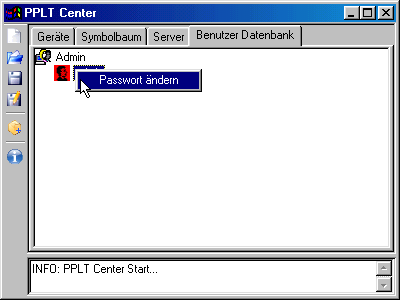
\includegraphics[scale=0.5]{chadminpass.png}
	\caption{Passwort des Administrators �ndern.}
	\label{fig:chadminpass}
\end{figure}

An dieser Stelle m�chte ich sie auf das eher eigenwillige Bedienkonzept des PPLT Centers
hinweisen. Wie sie sicher schon bemerkt haben, besitzt dieses Program kein Men�. Alle
aktionen werden mittels Kontextmen� initiert. Dieses �ffnen sie mit der rechten Maustaste.

\section{Allgemenies zur Oberfl�che}
Die Bedienoberfl�che des PPLT Centers besteht aus 3 Teilen. Dem ToolBar auf der 
linken Seite, mit dem sie eine Sitzung laden oder speichern k�nnen oder Module
installieren k�nnen. Der Zweite Teil ist das Log-Fenter,im unteren Teil des Programmes,
welches die (Fehler-)Meldungen der Bibliotek zeigt. Der Letzte und wichtigste Teil sind
die Reiter. Sie stellen die 4 Bereiche der PPLT dar. Zum einen die Ger�te und Server,
die sie laden und entladen k�nnen. Zum anderen der Symbol-Baum, in dem die Symbole 
verwaltet werden. Und zu letzt die Benutzerdatenbank mit der sie Benutzter und Gruppen
verwalten k�nnen. 

Im folgenden will ich mich auf die Bedienung und Funktion dieser Reiter beschr�nken. 
Dabei werde ich versuchen die Funktionsweise der PPLT anhand einiger Beispiele zu erkl�ren. 





%	\section{Ger�te Laden}
	Zu allererst sollten immer die Ger�te, die man ansprechen m�chte geladen werden.
	Dann sollten die Symbole erzeugt und mit den Ger�ten verbunden werden. Und zu letzt
	sollten die ben�tigten Server gestartet werden. Ich m�chte damit beginnen zu
	zeigen, wie im PPLT-Center Ger�te geladen werden. 
	
	Doch zu\-n�chst etwas Allgemeines. Die Ge\-r�te(-Dateien) sind der �ber\-sicht\-lich\-keit wegen
	in Gruppen unterteielt, die sich mei�t auf den Anwendungsbereich beziehen. So gibt es
	eine Gruppe \texttt{PLC}\footnote{PLC: \textit{eng.: Prgramable Logic Controler} 
	Speicherprogrammierbare Steuerung (SPS)} die alle Steuerungen zusammenfasst. 
	
	Um ein Ger�t zu laden, wechseln sie bitte auf den Reiter \texttt{Ger�te}. Dort
	sehen sie eine leere Lister aller geladenen Ger�te. �ffenen	sie mit der rechten 
	Maustaste das Kontextmen�\footnote{Dazu m�ssen sie sich mit der Maus �ber einen 
	leeren Bereich der Liste oder �ber dem Reiter selber befinden.}. Im Kontextmenu
	befindet sich nur eine Option "`Ger�t hinzuf�gen"'. W�hlen sie diese aus.
	
	Nun �ffnet sich die Ger�te-Auswahl. Dort sind alle bekannten Ger�te nach ihren
	Gruppen sortiert aufgelistet. Eine Gruppe �ffnen sie mit einem Doppelklick darauf.
	Bitte w�hlen sie mittels Doppelklick, das Ger�t \texttt{RandomGenerator} in der
	Gruppe \texttt{Debug} aus. 
	
	Die Gruppe \texttt{Debug} fasst alle Ger�te zusammen, die zum Testen der PPLT
	hilfreich seien k�nnen. Das Ger�t \texttt{RandomGenerator} simuliert ein
	reales Ger�t indem des Zufallswerte in verschiedene Typen Erzeugen kann. Da
	f�r dieses Ger�t keine real existierende Hardware von N�ten ist, werde ich
	es f�r die mei�ten der Beispiele verwenden. Was aber zu recht langweiligen
	Beispiel-Anwendungen f�hren wird. 
	
	\begin{figure}
		\centering
		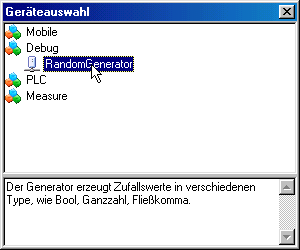
\includegraphics[scale=0.6]{DeviceSelection.png}
		\caption{Ger�teauswahl}
		\label{fig:DeviceSelection}
	\end{figure}
	
	Im unteren Teil der Ger�teauswahl\footnote{Siehe Abb(\ref{fig:DeviceSelection}).} 
	befindet sich ein kleiner Textbereich, indem eine kurze Beschreibung des 
	ausgew�hlten Ger�tes erscheint. Wenn eine �bersetzung f�r die von ihnen 
	eingestellte Sprache vorliegt, wird dieser Text	in der gew�hlten Sprache 
	ausgegeben.
	
	Zur Auswahl eines Ger�tes klicken sie bitte doppelt auf dieses. 
	
	Danach erscheint ein Dialog, mit dem sie die Parameter, die dieses Ge\-r�t
	be\-n�\-tigt. Auf jeden Fall fragt das System nach einem so genannten  Alias.
	Selbst wenn das zu ladenen Ger�t keinerlei Parameter ben�tigt. Dieser Alias 
	ist zur eindeutigen Identifikation eines jeden Ger�tes sowie eines Servers 
	n�tig. Sie k�nne ja schlie�lich mehrere Ger�te des selben Typs ansprechen
	jedoch bleiben dies unterschiedliche Ger�te. Es empfiehlt sich auch
	einen beschreibenen Alias\footnote{Man kann das Alias auch als eindeutigen
	Namen auffassen. Ich bezeichne es jedoch bewusst als Alias, da mit "`Ger�tename"' 
	eigentlich so etwas wie \textit{PLC.S7-200} gemeint ist. Also der Name des 
	Ger�tetyps.} auszuw�hlen um das Ger�t sp�ter besser identifizieren zu k�nnen.
	
	Da das Ger�t, der Zufalls Generator, den ich hier im Beispiel verwende keinerlei
	Parameter ben�tigt, fragt das System also nur nach dem Alias, wie in 
	Abb(\ref{fig:RandomSetup}) zu sehen ist.
	\begin{figure}[ht]
		\centering
		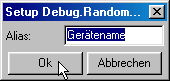
\includegraphics[scale=0.7]{RandomSetup.png}
		\caption{Setup des Zufallszahlengenerators}
		\label{fig:RandomSetup}
	\end{figure}
	
	
	Das Ger�t \textit{Debug.RandomGenerator} d�rfte sich problemlos laden lassen.
	Nun sollte das Ger�t in der Liste der geladenen Ger�te erscheinen 
	(siehe Abb.(\ref{fig:DevRand1})). 
	
	An dieser Stelle m�chte ich ihnen die Felder der Liste erleutern. Die erste 
	Spalte hei�t \texttt{Alias} und f�hrt die Aliases auf, die sie den 
	einzelnen Ger�ten gegeben haben. Die Spalte \texttt{FQDN} bedeutet 
	"`\textbf{f}ull \textbf{q}ualified \textbf{d}evice \textbf{n}ame"' 
	was �bersetzt so viel sagt wie "`Voll qualifizeirter Ger�tename"'.
	"`Voll qualifiziert"' bedeutet in diesem Fall, dass nicht nur der 
	Name des Ger�tes selber, sondern auch dessen Gruppe oder besser 
	Klasse mit angegeben wird. Dies dient dazu, das Gr�t wirklich 
	eindeutig zu benennen, schli�lich kann sich in einer anderen Gruppe 
	ein gleichnamiges Ger�t befinden. 
	
	Derelei Umst�ndlichkeiten wie diese, erscheint ihnen sicher erher 
	unn�tig. Wird aber vor allem dann wichtig, wenn ihnen kein 
	Auswahldialog, wie im PPLT-Center zur Verf�gung steht. Wie zum 
	Beispiel, wenn sie die PPLT als Python-Bibliothek	nutzten.

	\begin{figure}
		\centering
		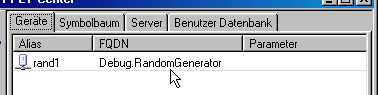
\includegraphics[scale=1.0]{DevRand1.png}
		\caption{Ger�teliste}
		\label{fig:DevRand1}
	\end{figure}	

	Die letzte Spalte tr�gt den Namen \texttt{Parameter}. In dieser Spalt, werden die
	Parameter, die sie dem Ger�t beim laden �bergeben haben, aufgelistet. Wie sie 
	erkennen k�nnen, ist dieses Feld beim Zufallsgenerator leer, da sie dem Generator
	keine Parameter �bergeben m�ssen.
	
\subsection{Ger�te mit mehreren Parametern}
	Neben dem Zufallsgenerator, der keine Parameter ben�tigt, gibt es nat�rlich auch 
	Ger�te, die mit Parametern geladen werden. Mit solchen Parametern, werden
	BUS- oder Netzwerkadressen, Time-Outs oder sonstiege Einstellungen get�tigt.
	
	Bei der auswahl der Parameter-Werte hilft ihnen ein verstekter Tool-Tip. Das
	sind keine Anzeigefelder, die erscheinen, wenn man mit der Maus �ber einem
	Objekt verweielt.
	
	\begin{figure}[ht]
		\centering
		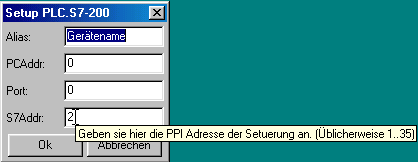
\includegraphics[scale=1.0]{S7Setup1.png}
		\caption{Tool-Tip f�r S7-200 Parameter}
		\label{fig:S7Setup1}
	\end{figure}
	
	In der Abbildung (\ref{fig:S7Setup1}) sehen sie den Parameter Dialog, 
	f�r die Simatic S7-200 	Ger�teunterst�zung. F�r den Parameter 
	\texttt{S7Addr} ist der Tool-Tip zu sehen, der erkl�rt, was es mit diesem
	Parameter auf sich hat. Mei�t sind die Parameter mit Standardwerter vorbelegt,
	die sie nur noch auf ihre Bed�rfnisse anpassen m�ssen.


\section{Ger�te Entladen}
	Da sie nun in der Lage sind Ger�te zu laden, haben sie sicher auch interesse diese 
	wieder zu entladen. 
	
	\begin{figure}[ht]
		\centering
		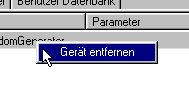
\includegraphics[scale=1.0]{DevDel.png}
		\caption{Ein Ger�t entfernen.}
		\label{fig:DevDel}
	\end{figure}
	
	W�hlen sie dazu das zu l�schende Ger�t aus und �ffnen sie mittels Rechtsklick
	dessen Kontextmen�. Dieses Men� enth�lt lediglich den Eintrag "`Ger�t entfernen"'.
	Klicken sie darauf um das Ger�t zu entfernen.
	Wenn keine Fehler auftreten wird das Ger�t aus der Liste gel�scht.
	
	%\input{SymbolTree}
	%\input{StartServer}
	%\input{UserDB}

%\chapter{PPLT Referenz}
%\chapter{pyDCPU Referenz}
\chapter{PPLTServer und Device Referenz}
	Dieses Kapitel beschreibt den Syntax der Ger�te- und Serverdateien. Sie bilden 
den wichtigsten Teil der PPLT Abstraktionsschicht. Diese Beschreibungsdateien
im XML Format enthalten die Informationen, wie das System vorhandene Kernmodule
miteinander kombinieren muss, um ein Bestimmtes (reales) Ger�t anzusprechen oder 
einen bestimmten Dienst\footnote{Server} zur Verf�gung stellen kann.

Die Server und Ger�tedateien besitzen immer den selben Aufbau. Hier am Beispiel einer
Ger�tebeschreibungsdatei.

\begin{verbatim}
<?xml version="1.0"?>

<PPLTDevice name="Steuerung">
	<Head>
		<Description>...</Description>
		<Require>...</Require>
		<Provide>...</Provide>
	</Head>
	
	<Setup>
		...
	</Setup>
</PPLTDevice>
\end{verbatim}

Alle f�r das Ger�t relevanten Informationen sind in den \texttt{PPLTDevice}\footnote{Beim Server
hei�en diese \texttt{PPLTServer}.} Klammern eingeschlossen. Die Informationen werden in einen
Kopf (\texttt{Head}) und einen Setupbereich aufgeteielt. Im Kopf befinden sich alle beschreibenden 
Informationen wie einem kurzen Text, der das Ger�t und dessen Funktionen 
erleutert\footnote{\texttt{Description}}. Einem Block, der die Voraussetzungen, die dieses Ger�t 
ben�tigt\footnote{\texttt{Require}} beschreibt sowie einem Block indem alle Anschl�sse\footnote{Slots},
die das Ger�t beitet\footnote{Provide} auflistet.

Ich werde im folgenden den Aufbau der Beschreibungsdatei recht technisch aufschl�sseln. Es ist daher
eine Gewisse Vorkenntnis der PPLT von N�ten um die Ausf�hrungen verstehen zu k�nnen.

\section{\texttt{PPLTDevice} \texttt{PPLTServer}}
Innerhalb dieser Tags werden alle relevanten Informationen, die zur Beschreibung der Servers oder
des Ger�tes dienen, aufgelistet. Dieses Tag besitzt ein notwendige Attribute. Die Angabe dieser 
Attribute ist Pflicht.

\begin{tabular}{c|l}
\texttt{name}		& Gibt den Namen des Ger�tes oder des Servers an.\\
\texttt{class}	& Gibt den Namen der Klasse an, der dieses Ger�t oder Server zugeordnet werden soll.\\
\texttt{version}&	Gibt die Versionsnummer des Ger�tes an. 
\end{tabular}



\section{\texttt{Head}}
	Im Head werden wie Anfangs schon erw�hnt beschreibene Informationen zum Ger�t oder 
	Server aufgelistet. Immerhab der \texttt{Head}-Klammern d�rfen lediglich Elemente
	vom Namen \texttt{Description}, \texttt{Require} oder \texttt{Provide} stehen.
	
	Das Tag \texttt{Head} ben�tigt keinerlei Attribute.
	
\section{\texttt{Description}}
	Das Tag \texttt{Description} kann innerhalb vieler Tags verwendet werden, es enth�lt immer
	eine kurze Beschreibung des Kontextes, indem es steht. 
	
	Das \texttt{Description}-Tag kann innerhalb der Klammern \texttt{Head} und \texttt{Variable}
	stehen. Wenn das Tag im Kontext \texttt{Head} verwendet wird, kann damit dem gesamten Ger�t
	ein beschreibender Text gegeben werden. Wird das Tag im \texttt{Variable}-Kontext verwendet
	wird einer bestimmten Variable eine Beschreibung zugeordnet.
	
	Als Attribut muss dem \texttt{Description}-Tag immer \texttt{lang} �bergeben werden. Damit
	wird die Sprache des Beschreibungstextes fest gelegt. 	
	
\section{\texttt{Require}}
	Innerhalb der dieser Klammern, werden alle Voraussetzungen, die das Ger�t oder der Server
	ben�tigt aufgelistet.	
\section{\texttt{Setup}}




\end{document}
